\documentclass[12pt,a4paper]{article}
%packages usage
\usepackage[left=20mm, top=20mm, bottom=20mm, right=20mm]{geometry}
\usepackage[utf8]{inputenc}
\usepackage{multicol}
\usepackage{amsmath}
\usepackage{graphicx}
\usepackage{xcolor}
\graphicspath{{./graphic/}}
%title page
\author{instructor: Dr.Sven Kuhn \\ student: Thanh Toan Truong}
\title{Development Of A Wireless Shoe\\Senior Project Report}

\begin{document}
\maketitle
\pagebreak
\begin{abstract}
Mechanical and robotic development has exceeded the level of control for functional robots links,joints that can achieve the dexterity and precision even more than that of a living organism. A large number of robots now are inspired from animal, especially ones with limbs, including human. Yet there are still limitation of how alike and natural the movement should be, so that it can replace, for example, broken or handicapped limbs. This can be overcome by pursuing the study of the living body by examining humanoid movement. Because of that, this report examine a candidate prototype of a system, named \textit{"Wireless Shoe"} to collect the plantar and acceleration data around the foot area of a human left leg. Afterwards, this prototype can be used to realize a more compact Printed Circuit Board (PCB) for installation onto the shoe to collect the data.
\end{abstract}
\pagebreak
\tableofcontents
\pagebreak
%================================================================D
\section{Introduction}
The goal of this project is to realized a device that can be attached to the shoe, then send wireless data to a computer. The name of the project-\textit{Wireless shoe}, imply the usage of one shoe as the carrier of the device and as the subject for collecting data. Throughout this report, a prototype circuit for the WS system was designed and reviewed. Some discussions are included for further development of the system. This report is written due to the requirement of the last semester's senior project, EEIT Bachelor program at Frankfurt University of Applied Sciences, in the exchange study period from Vietnamese German University.
The working period for this report 23/04/2019 - 20/05/2019 was carried out in order to realized a prototype for the "Wireless shoe" system.
\section{Design of the system}
\hspace{10mm}This section covers the proposed design of the device, data type, how to measure them and the process of making the prototype of the Wireless Shoe system. The device was not full design in the last period, but for some potential placements of the system on a shoe, one may refer to Figure 1:
\begin{figure}[hbt!]
\begin{center}
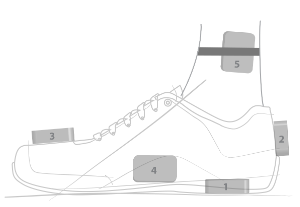
\includegraphics[scale=1]{SPlacement.png}
\caption{Some variation of where the device can be put \cite{Splacement}}
\end{center}
\end{figure}
\subsection{Which data to take}
\hspace{10mm} With the ever increasing rate of processor speed and new data processing algorithm, It is both ambitious and reasonable that the device should get the most data as it could. Most systems made for this type of measurement are implemented around either Acceleration, Ground reaction force or Acceleration\cite{acc1,And03astudy}. The "Wireless shoe"(WS) system thus, is keen to collect the data of all types: Acceleration, Angle velocity and Ground Reaction Force with respect to time, see Figure 2 for the data block, which is constructed and sent by the device.\\
\begin{figure}
\begin{center}
\begin{tabular}{|c|c|c|c|c|c|c}
	\hline
	Flexiforce A301 & Gyroscope & Accelerometer & Esp8266\\
	\hline	
	FSD0 ... FSD5 & AVx AVy AVz & ACx ACy ACz & timeStamp\\
	\hline
	16 bit integer&angle rad/s&acceleration $g/m^2$&ms\\
	\hline
\end{tabular}
\end{center}
\begin{tabular}{l l}
FSD0 ... FSD5	& selected 6 sensors for ground reaction force\\
AV(x,y,z)    	& the gyroscope measurement from MPU6050\\
AC(x,y,z)    	& the accelerometer from the MPU6050
\end{tabular}
\caption{\textit{Data block for each measurement}}
\end{figure} 
\subsection{Implementation}
\hspace{10mm} To collect data of a moving subject, it is preferred to use a wireless system, allowing the subject to move freely around, permitting natural pose and gesture. A study suggests that immobilized walking for example with a treadmill might cause unnatural gait\cite{And03astudy}.For developing the Wireless Shoe system, A prototyping system to evaluate the combined operation of different sensors type was designed:
\begin{enumerate}
\item A local Java Socket Server running on a laptop collects the data from the device, which was attached to the shoe. Afterwards, the data are stored in a text file with the data readings and its respective time stamps.
\item A separated device/PCB to be attached to the left sneaker, sending collected data to the server. 
\end{enumerate}
This design is realized in the time this report is written as the first prototype of the Wireless Shoe system. Further processing are not included and saved for later work. Due to the lack of time, this prototype wasn't finished and have realized errors, which were not solved. However, This work was able to check the sensors' functionality, the wireless function and pointed out some drawbacks of the design.  
\subsubsection{Proposed Circuit}
\begin{figure}[hbt!]
\includegraphics[width = 170mm]{full_circuit.png}
\caption{Proposed Circuit for WS system}
\end{figure}
\begin{enumerate}
  \item \textit{Power Input} \\
The intention of the WS system power supply is to last for at least more than a soccer match, so that it could be used by plaer to collect the match data. In Soccer, a normal game takes about 90 minutes \cite{lawOfTheGame}, 15 minutes for the half-time break, plus 15+15+5 minutes for the out-time match and around 20 minutes for the penalty round. These period result in a total of approximately 2 hours and 40 minutes.
\begin{equation}
	T_{operating}=90+15+15+15+5+20=160\:[minutes]
\end{equation}
To calculate the necessary battery capacity, a total operating current was approximated by summing all operating current of the modules in the System, except for the laptop \cite{Esp8266,ADS1115,MPU6050,LM358}. 
\begin{center}
\begin{equation}
I_operating=80mA+300\mu A+500\mu A+3.6mA+1.2mA=85.6mA
\end{equation}
\begin{tabular}{ |c|c|c|c|c|}
\hline
Wemos D1 mini Esp8266-12F & ADS115 & MPU6050 & LM358 \\ 
\hline
80 mA & 300 $\mu$A & 500 $\mu$A + 3.6 mA  & 1.2 mA\\
\hline
\end{tabular}
\end{center}
Battery capacity calculation:
\begin{equation}
	Capacity\:=\frac{160}{60}\times85.6=\:\approx\:228.26\:mAh
\end{equation} 
It is always preferable to choose a slightly higher capacity than that the system need, as the full test of the system was not carried at the time. But about 400-800 mAh would be a sufficient choice. Additionally, rechargeable power source is better, so that the WS system can opt out of battery replacements every run.\\
It is worth pointing out that the ESP8266-12F (ESP) account for most power consumption of the system and 80 mA is only the average operating current. Some experiments also showed a current surge at the booting stage of the ESP \cite{EspPower1}\cite{EspPower2} of around 150-300 mA in microseconds. The power supply then should be able to withstand this phenomenon.\\
The battery used in this prototype system was a 18650 model Lithium-Ion battery, for ease of usage and rechargeability. The 3.7v battery can support $\approx$ 2000mAh of capacity\cite{18650}, which is now an overkill for our application. However, it comes with assurance that the battery would provide enough power for the system, see figure 4\footnote{Figure 4 of the batter dimension was edited by the writer to better fit the report, \textit{software: Photoshop Cs6}}.

\begin{figure}
\begin{center}
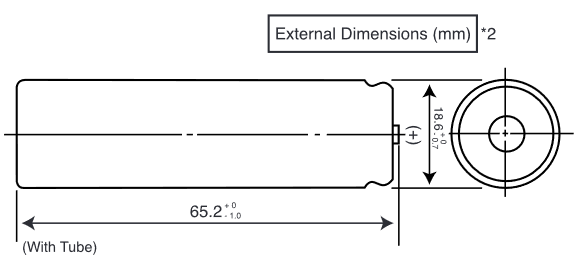
\includegraphics[scale=0.7]{18650.png}
\caption{18650 battery - courtesy from Panasonic\cite{18650}}
\end{center}
\end{figure}
To make the power supply, the battery was fed to a 3.3V voltage regulator, powering all modules in the system. The chosen regulator at the moment was AMS1117-3.3 module, See Figure 5\\
\begin{figure}
\begin{center}
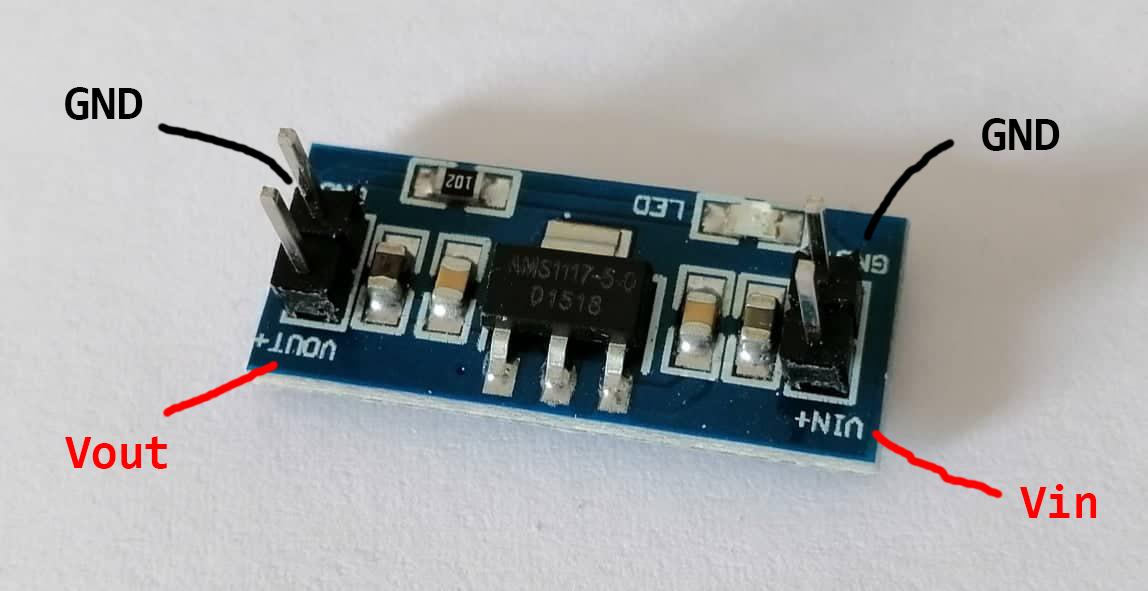
\includegraphics[width = 100mm]{AMS1117.png}
\caption{3.3V Voltage Regulator AMS1117}
\end{center}
\end{figure}
A parallel Capacitor 470$\mu$F was added to eliminate high frequency voltage bounce when the switch is triggered See Figure 3.
  \item ADS1115 Analog Digital converter\\
\hspace{10mm}The readings of the Force sensor was supposed to be carried by the ADS1115s Analog-Digital converter(ADC). With 16 bit, high range($\pm$6,144v) reading, it was chosen to compensate for the Esp8266 10bits low range(0-1v) ADC. At the time this report was written the ADS1115 was not available, thus its operation are omitted from the scope of the evaluation now, a section will still be kept to imply its usage. The sensors were tested with a multimeter on a seperate circuit.
  \item A301 Tekscan force sensor\\
For the measuring of the ground reaction force, the selected sensor should be slim enough to be installed on the insole, versatile and have a range big enough for human weight. Because of its compact size and weight range, 6 TekScan A301 Force sensors, Figure 2 and 7, were employed for the job\footnote{This analysis was earlier informed to me by my senior, he gave me the sensors, which I stripped from one of his failed product.}.\\
It has the measure range of 445N (0-100lb), thickness of 0.203mm \cite{A301}. Although the average body mass globally was about 62kg (study made in 2012 \cite{weight}), most of the body mass lays on the sensor distribute through the shoe's cushion and through the much larger area of the insole. This leaves the sensors to be subjected by a smaller force from the body mass.\\
The proposed circuit for measuring the Force sensors was referred from TekScan Flexiforce A301 datasheet\cite{A301},See figure 3 and 6.\\
Each sensor's circuit will be tweaked later with a potentionmeter, so that a strongest reasonable force for each one in operation can be realized and collected. And maximum voltage reading should be in the data range of the ADS1115, which was proposed $\pm2.048V$ with power supply 3.3V. For the input voltage of the sensor, we will go for about -1V.\\
Another problem was raised here, that a negative voltage,or a dual-supply needs to be realized to power the Op-Amp. The independent circuit to check the functionality of a sensor was carried out, see Figure 11 section Current Result. 
\begin{figure}[hbt!]
\begin{center}
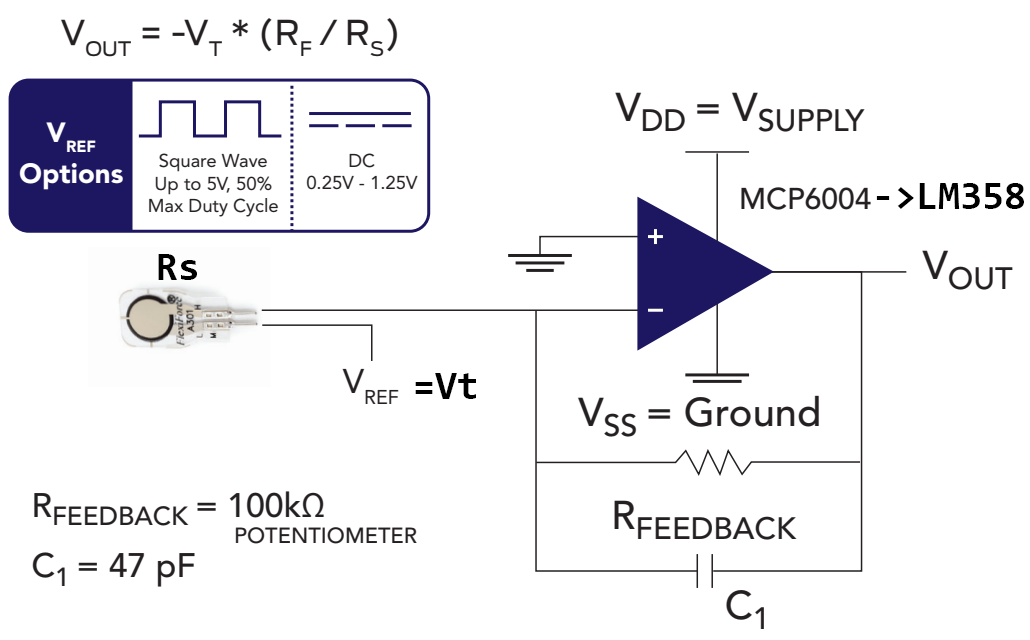
\includegraphics[width = 170mm]{A301.png}
\caption{Proposed circuit from Tekscan\cite{A301}}
\end{center}
\end{figure}
\begin{figure}[hbt!]
\begin{center}
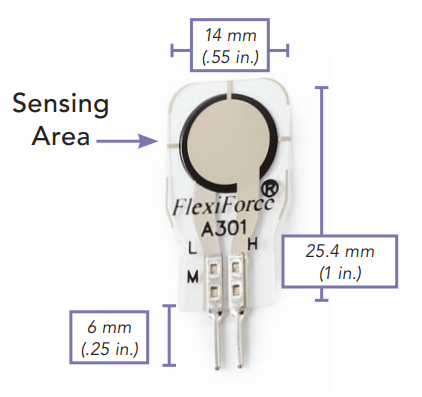
\includegraphics[scale=1]{flex.png}
\end{center}
\caption{A301 Force sensor - Picture from TekScan\cite{A301}}
\end{figure}   

  \item MPU6050\\
To collect the Acceleration and Angle velocity from the foot, the development module MPU6050 was used. With capabality up to $\pm$16g of XYZ accelerometer and $\pm$2000$^o/s$ as XYZ angle velocity sensing, MPU 6050 is a suitable choice for the project.\\
The Module uses I2C interface to send the data to Esp8266. The data is then processed to the data block in Figure 2. Collection of Acceleration and Angle velocity can be referred to an earlier work from \cite{acc1}, which also included an method for processing of collected data. The chosen module of interest was GY-25, however, It is not clear that because of the code library, or that it was damaged during soldering, the data from the module (acceleration and angle velocity)was not readable from I2C interface. The data was read through Tx and Rx (Serial)\cite{GY25}, and only value of Yawn, Pitch and Roll (can be transferred to angle velocity) can be read. Though the datasheet of MPU6050 points out that it has accelerometer imbued in the Chip\cite{MPU6050}. Most application for the GY-25 regard it as a "tilt angle module". The earlier intention should points to another module GY-521, which has a better supported library.\\
Currently the GY-25 is set to communicate with Esp8266 through Serial (TX,RX) port.For this reason, the Tx,Rx connecting wires need to be unplugged every time a new code was uploaded to the Esp8266. Data of the Gy-25 are represented as Roll - Pitch -Yaw depicted in figure 8.
\begin{figure}
\begin{center}
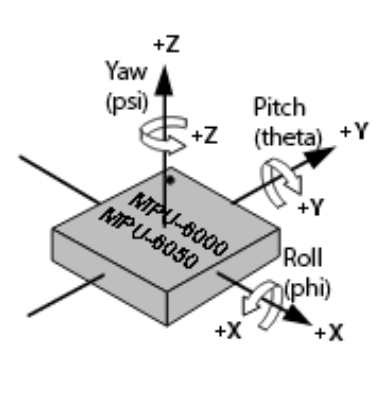
\includegraphics[width = 70mm]{rpy.png}
\hfill
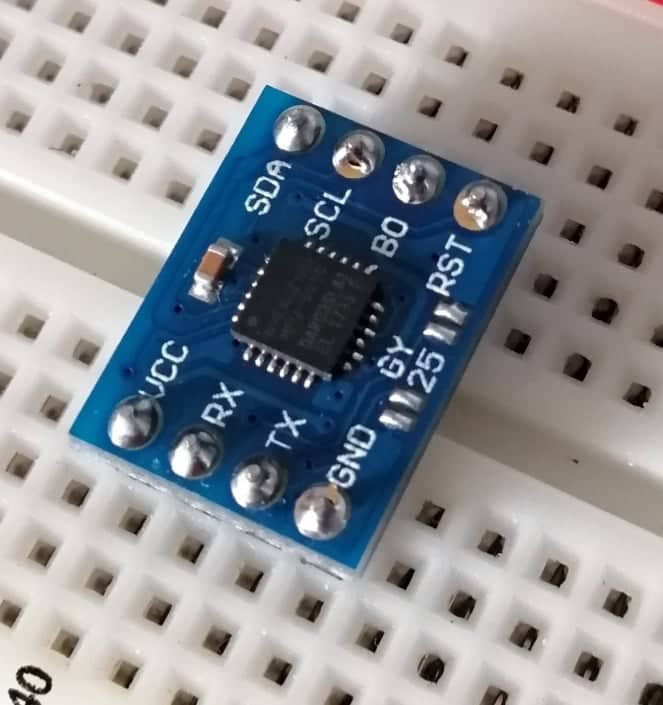
\includegraphics[width = 80mm]{Gyro.jpg}
\caption {Data representation in $^o$-degree of the GY-25 }
\end{center}
\end{figure}
 
  \item ESP8266\\
The module Wemos d1 mini, with Esp8266 play the roll of the data block (see Figure 2) constructor and transmitter. The code on Esp8266 was made and uploaded by Arduino IDE 1.8.9. In Operation Esp8266 first initialized all modules into reading mode. Then It construct a String of collected data. This data then is sent to the Java Socket server on the laptop and store in a text file, the reading was set to read the data for 30s.   
For the power source, the Wemos d1 module can tolerate a voltage from 3v to 5v. The power source was connect to G and 5V on the module. The two I2C pin for communicating with ADS1115 was D1-SCL and D2-SDA.\\	
\begin{center}
\begin{tabular}{|l|l|l|l|}
	\hline
	5V & G & D1 & D2\\
	\hline
	Vcc&Gnd& SCL&SDA\\
	\hline
\end{tabular} 
\end{center}
\end{enumerate}
\subsubsection{Operation}
To operate the Data transferring of the Esp8266, a local area network had to be opened on the laptop. The laptop then run the Java program and wait for the Esp8266 to connect to the server and start recording signal. After 30s, the Esp8266 stopped sending data. The record was stored in a text file \textit{tes.txt} in the same directory of the java program. The data can be accessed from the file.\\ 
For the purpose of prototyping, the system was only worked on a bread board with two separate tests : the Esp8266 with GY-25 and the A301 force sensors. The Esp8266 and GY-25 worked with the procedure above. The A301 force sensors in the other hand did not worked as planned, more information are available in Current Result.\\
Additionally, to attached the sensor to the shoe, an special insole was made from rubber sheet, cut in the form of an normal insole, see figure 9. The sensors should be then mounted on the insole to be put under plantar pressure.\\
\begin{figure}
\begin{center}
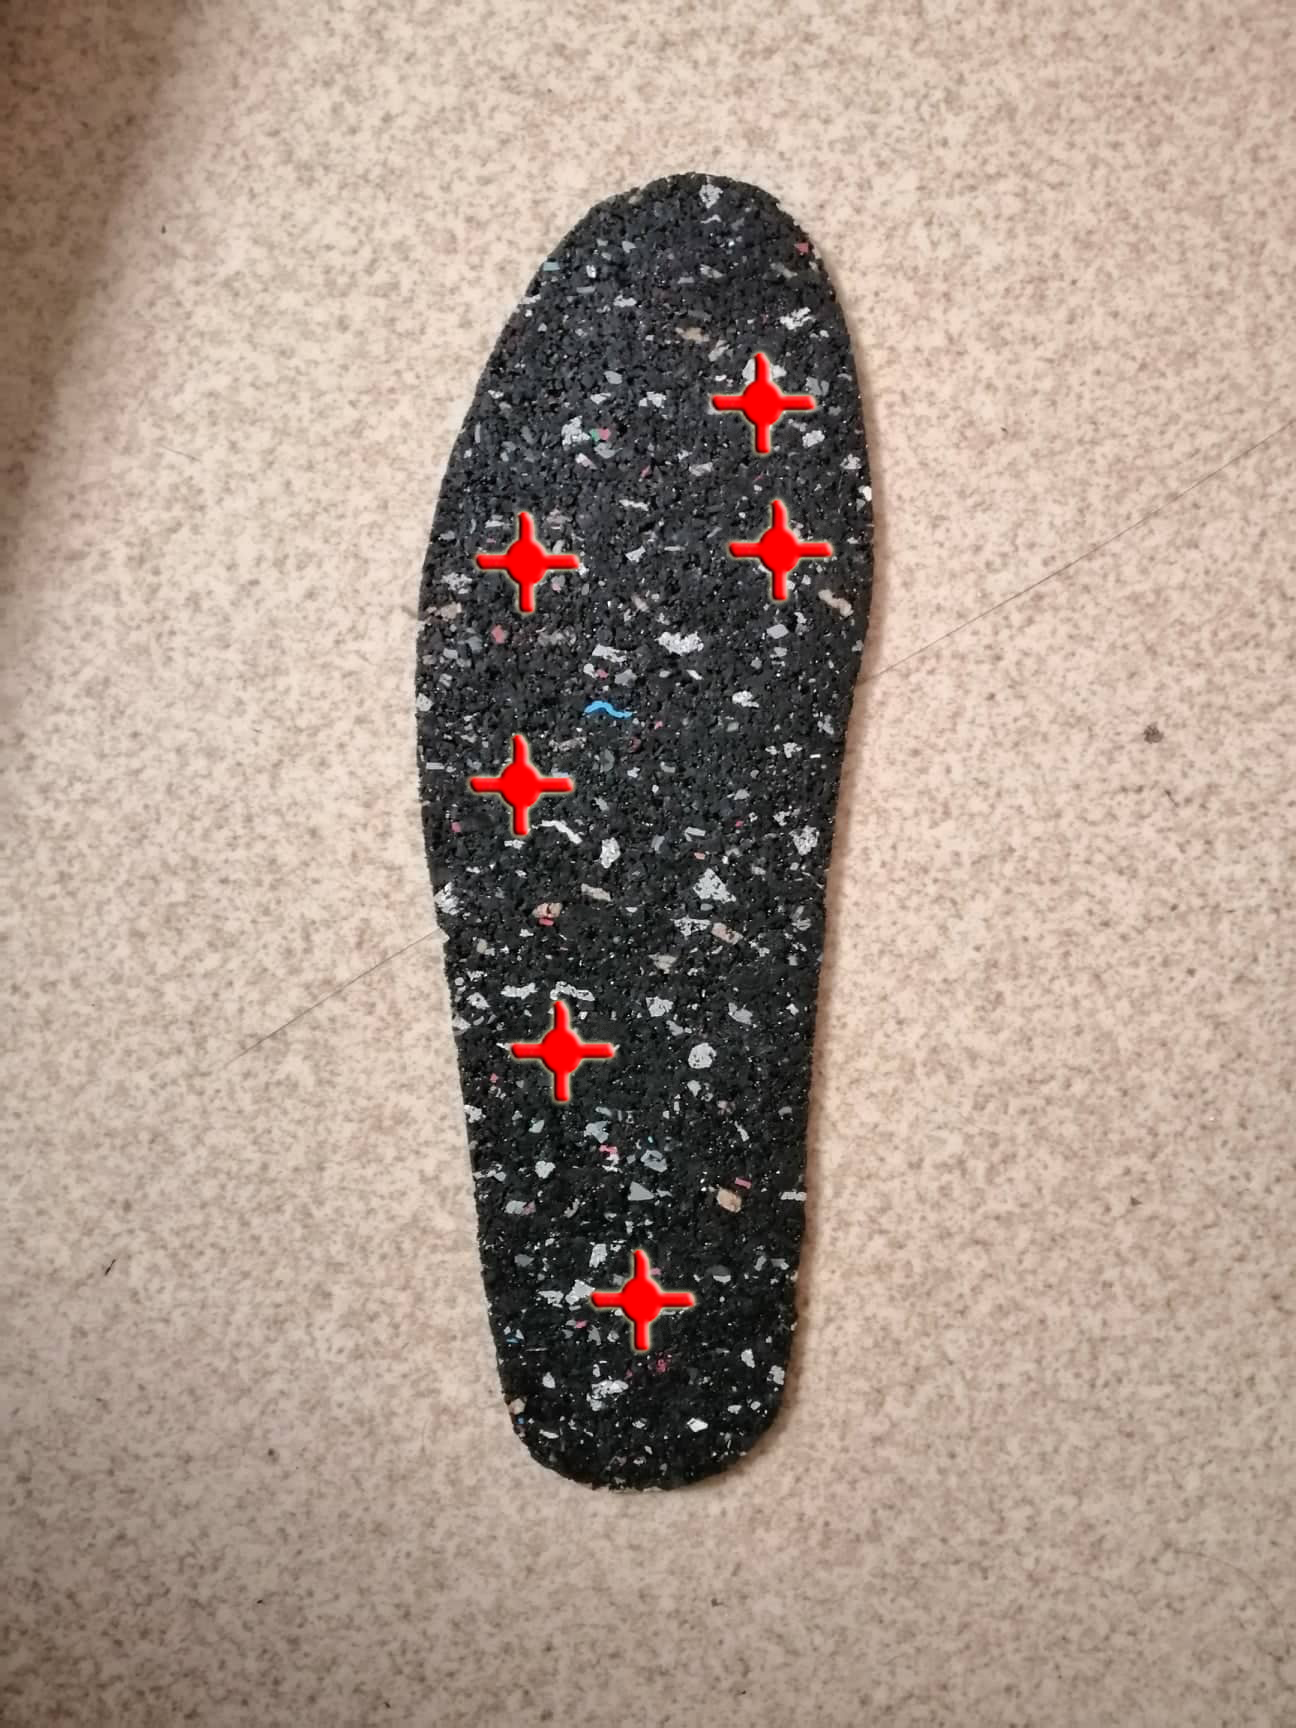
\includegraphics[width = 70mm]{insole.png}
\caption{the insole and placing position of sensors}
\end{center}
\end{figure}
\section{Current Result}
\subsection{Data Transferring}
The data transferring module of the Wireless Shoe system work quite well at the moment, for the usage of tcp-ip ensured the reliability of the data. The Excel plotting with time stamps can be observed in Figure 10.
\begin{figure}
\begin{center}
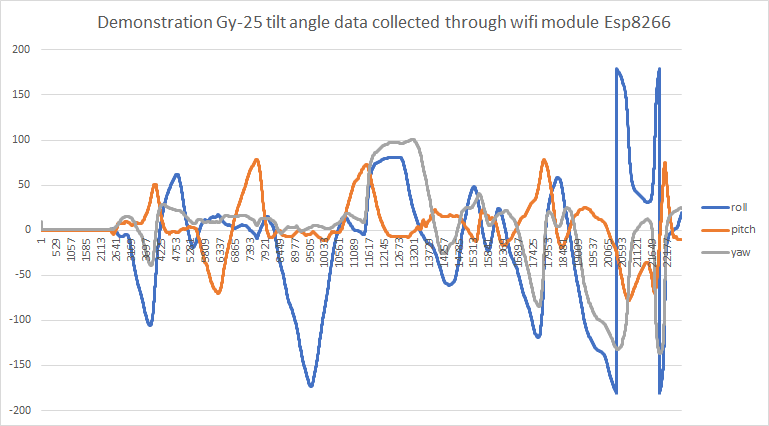
\includegraphics[scale=1]{Gy25}
\caption{data collected - only data from the gyroscope tilt-angle representing Roll-Pitch-Yaw}
\end{center}
\end{figure} 
\subsection{Ground reaction force data collection}
A complete combination test of the system was not carried out due to absence of component(ADS1115 ADC) and the realization of the dual power (Vcc and Vee) supply for the Op Amp.\\
The proposed circuit prove the working principle of the Ground reaction force sensor TekScan Flexiforce A301, see figure 11.
\begin{figure}[hbt!]
\begin{center}
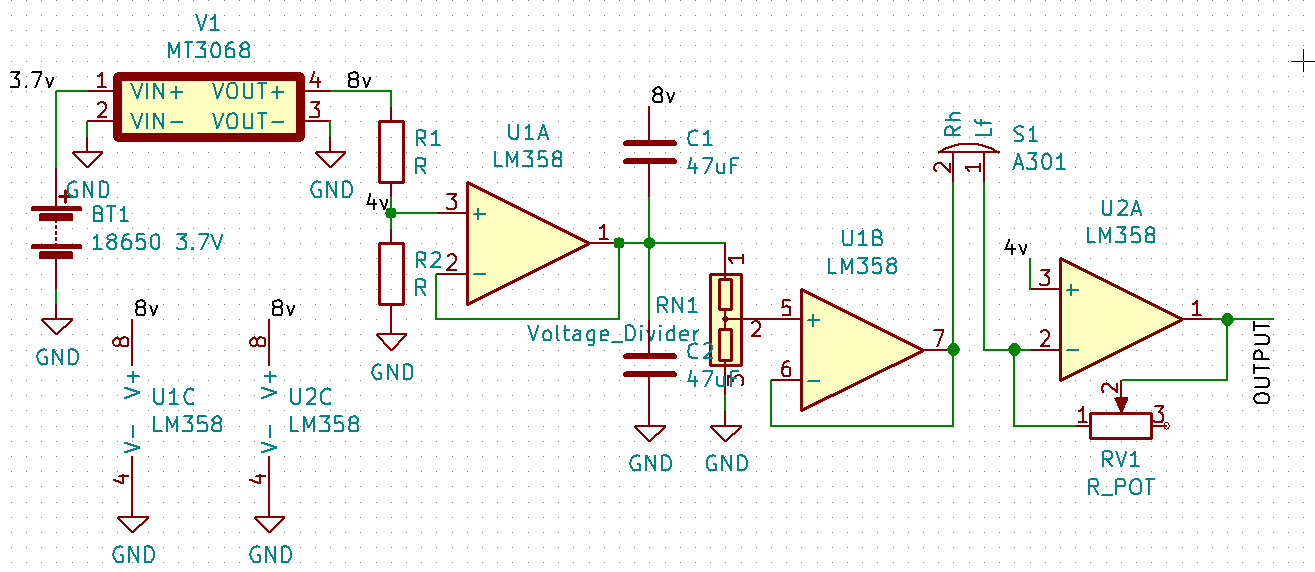
\includegraphics[width = 170mm]{lm358test.png}
\caption{Testing circuit for one force sensor}
\end{center}
\end{figure}
Because the unavailability of a dual supply, the tesing circuit used an 8v power source and the voltage divider of R1 and R2 to separate itself into 3 voltage level 8v, 4v, and 0v. The 4v was considered as virtual ground-GND. 2 LM358s were used for signal-conditioning. Total of 3 Op-Amp (3/4) from the LM358s were used in the circuit. The fist Op-Amp, from the left, was employed as a non-inverting voltage follower to transfer the referencing virtual ground (GND/4v) to avoid chaging impedance at the first part of the circuit. The output reference was connected to a potentionmeter to generate new reference voltage, $-\:1V$, for the sensor, see figure 6. The new reference voltage was fed to the second Op-Amp, also a non-inverting voltage follower, to keep the voltage without changing the impedance of the left side of the circuit. The voltage was then applied to the sensor. The last Op-Amp functioned as a inverting voltage amplifier, taking the signal from the sensor as inverting input. The second LM358 ran on the power of virtual 4V/8V and virtual ground/4V, the non-inverting was connected to virtual ground/4V. The last output signal is measure with reference to virtual ground as a positive value, see Figure 11,12.\\
\begin{figure}[hbt!]
\begin{center}
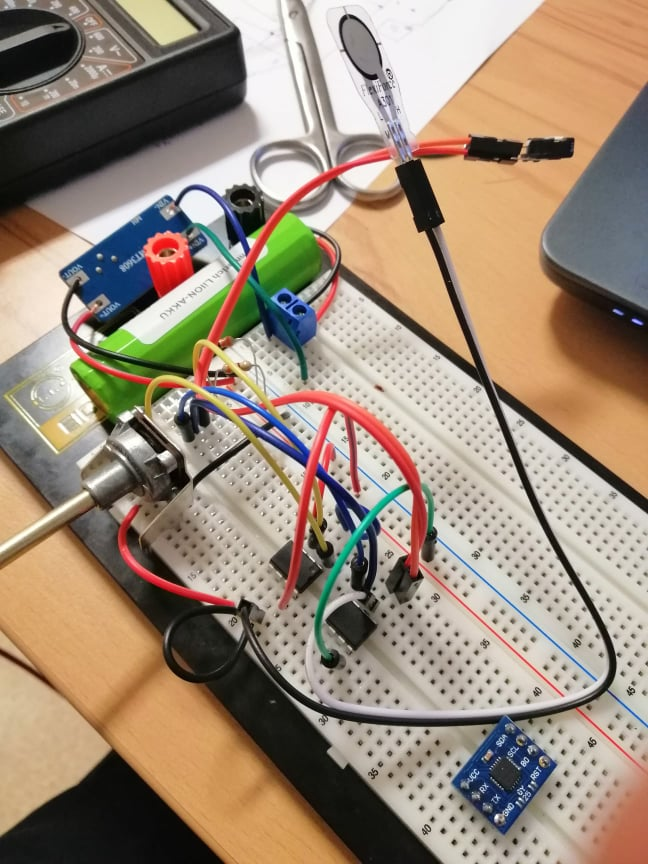
\includegraphics[width = 170mm]{test1.jpg}
\caption{circuit attempt to collect the sensor data}
\end{center}
\end{figure} 
The circuit didn't work as expected, the final output did change with respect to change of pressure acting on the sensor. But the voltage is negative with respect to virtual ground/4V. The stronger the pressure, the higher amplitude the voltage different.
\subsection{Insole}
The insole was built and fit perfectly into the shoe, Figure 9. The sensors were not yet attached because the system was not complete in the time this report is written.
\subsection{MPU6050}
The tilt angle - angle velocity data collecting worked fine. The data collected was successfully sent, received and stored in a text file, a graph-Figure 10 was plotted in Excel to show the data when the system was wielded around in mid air\footnote{It is like playing the breadboard as an airplane}. The maximum read are 180$^o$ and -180$^o$, these are angle with respect to the initial start-up orientation.\\
The acceleration data was not yet collected. 
\section{Discussion}
Although this Prototype cannot fulfill the requirement of the Wireless shoe system in term of physical and sampling rate, It can still be used in aid of testing the new components and mark the milestone from with the system can be further developed.
\subsection{Power source}
With the referenced fixed cylindrical shape and weight around 45g \cite{18650}, it is unlikely that this battery can be appropriate for athletic motion such as running,sprint or even jogging, not mentioning playing soccer. Some super-capacitor design \cite{newbat} may benefit this WS system, as for paper-slim thickness and versatile operation, see Figure 13.\\
Apart from Lab battery, a slightly different Lithium battery from today smartphone and Portable device, with thinner design, may be a good replacement for the 18650. The phone's battery wasn't used in this report due to the purpose of prototyping, safety and time restriction.
\begin{figure}[hbt!]
\begin{center}
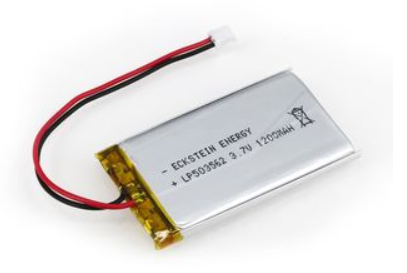
\includegraphics[width = 85mm]{lipo.png}\hfill
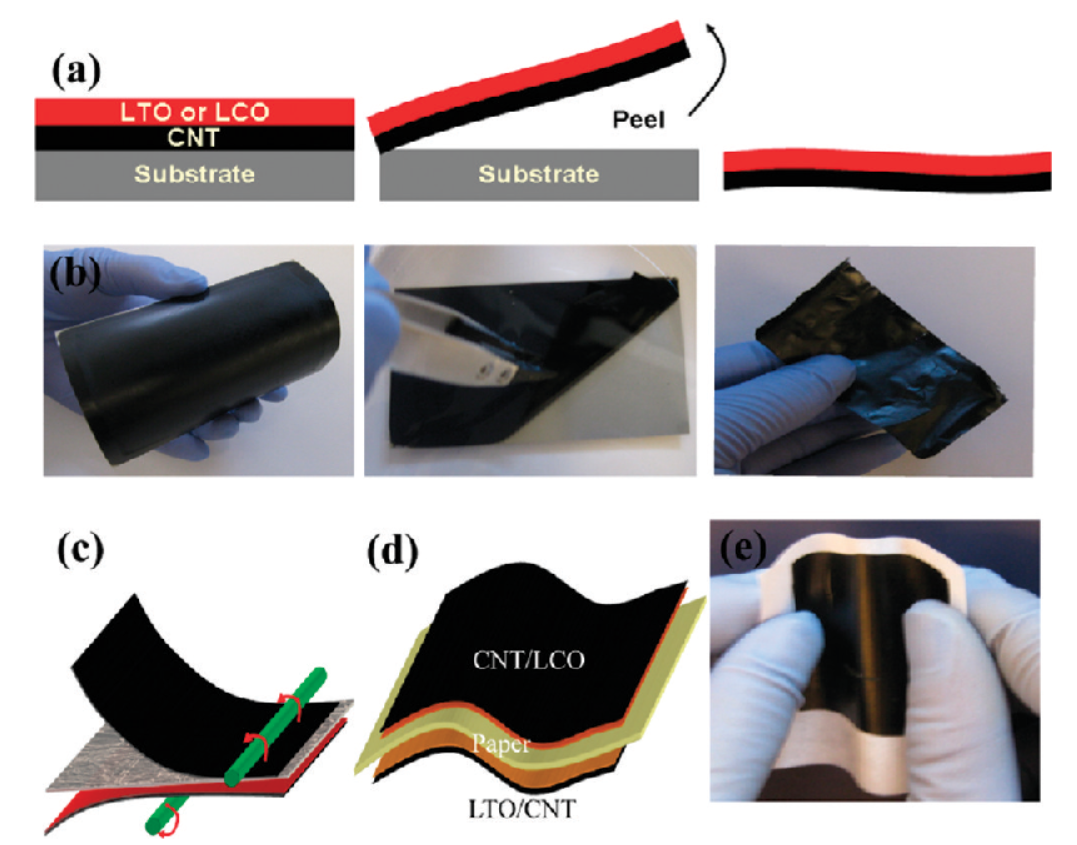
\includegraphics[width = 85mm]{paperbat.png}
\caption{Lipo battery from Eckstein Komponente(left), Paper battery structure(right)\cite{paperbat}}
\end{center} 
\end{figure}
\subsection{Dual Supply voltage}
Work should be done further to realize a dual supply voltage. This may solve the problem of the ground reaction force data acquisition.
\subsection{Gyroscope and Accelerometer}
The Gyroscope or tilt angle module by far works very well. Further work would then include realization of the Accelerometer either from the GY-25 or to use a different module, GY-521 for example.
\section{Conclusion}
For the final recap, a prototype for the system has been realized, the functionality of the sensors were also tested. The discussion section shows how the system might be enhanced for more performance and what is left to complete the full prototype.\\
Through the working period, many of the knowledge gained from the study program were applied : Op-Amp design,PCB design, soldering, Micro-controller Programming and Report writing.\\
Further works include the testing the whole design with ADS1115, the realization of the smaller PCB - design of the system, processing of collected signal and field test.
\begin{thebibliography}{991}
\bibitem{lawOfTheGame}
\textit{Laws Of The Game 2019,Law 7-The Duration of the Match}, The International Football Association Board, accessed 15 May 2019,$<$http://theifab.com/laws$>$.
\bibitem{Esp8266}
Espressif System,\textit{"ESP8266EX"},\textit{ESP8266 Wifi module datasheet},version 6 [revised November 2018], accessed 15 May 2019.
\bibitem{EspPower1}
\textit{Determining the ESP8266 power consumption}, web article , 2017-02-	07 by Ondřej Hruška, acessed 15 May 2019, $<$https://www.ondrovo.com/a/20170207-esp-consumption/$>$
\bibitem{EspPower2}
Current consumption analytics on ESP8266 for battery users, ESP8266 Community Forum,From dkdileep posted on 3 Jul 2015, accessed 15 May 2015.
\bibitem{ADS1115}
Texas Instruments,\textit{"ADS111x Ultra-Small, Low-Power, I2C-Compatible, 860-SPS, 16-Bit ADCs.
With Internal Reference, Oscillator, and Programmable Comparator", ADS1115 datasheet}, SBAS444D-May 2009 [revised Jan. 2018], accessed 15 May 2019.
\bibitem{LM358}
Texas Instruments, \textit{"LMx58-N Low-Power, Dual-Operational Amplifiers", LM358 datasheet}, SNOSBT3I –JANUARY 2000, revised Dec. 2014, accessed 15 May 2019.
\bibitem{MPU6050}
InvenSense,\textit{"MPU-6000 and MPU-6050 Product Specification Revision 3.4", MPU6050 datasheet},Release Date: 08/19/2013, accessed 15 May 2019.
\bibitem{18650}
Panasonic,\textit{LITHIUM ION BATTERIES: INDIVIDUAL DATA SHEET, CGR18650DA: Cylindrical Model}, Jan 2007, accessed 17 May 2019
\bibitem{A301}
TekScan,\textit{"FlexiForce™ Standard Model A301", A301 data sheet},DS Rev F 101518, accessed 15 May 2019.
\bibitem{And03astudy}
Rawesak Tanawongsuwan And and Rawesak Tanawongsuwan and Aaron Bobick, A Study of Human Gaits across Different Speeds, 2003,accessed 15 May 2019.
\bibitem{weight}
Walpole, Sarah \& Prieto-Merino, David \& Edwards, Phil \& Cleland, John \& Stevens, Gretchen \& Roberts, Ian. (2012). The weight of nations: An estimation of adult human biomass. BMC public health. 12. 439. 10.1186/1471-2458-12-439. 
\bibitem{Splacement}
J. Doppler et al., \textit{"Variability in Foot-Worn Sensor Placement for Activity Recognition,"} 2009 International Symposium on Wearable Computers, Linz, 2009, pp. 143-144.
doi: 10.1109/ISWC.2009.18
\bibitem{newbat}
Hu, Liangbing \& Choi, Jang \& Yang, Yuan \& Jeong, Sangmoo \& La Mantia, Fabio \& Cui, Li-Feng \& Cui, Yi. (2009). Highly conductive paper for energy-storage devices. Proceedings of the National Academy of Sciences of the United States of America. 106. 21490-4. 10.1073/pnas.0908858106. 
\bibitem {paperbat}
Hu, Liangbing et al. “Thin, flexible secondary Li-ion paper batteries.” ACS nano 4 10 (2010): 5843-8 .
\bibitem {acc1}
S. Ding, X. Ouyang, T. Liu, Z. Li and H. Yang, "Gait Event Detection of a Lower Extremity Exoskeleton Robot by an Intelligent IMU," in IEEE Sensors Journal, vol. 18, no. 23, pp. 9728-9735, 1 Dec.1, 2018.
doi: 10.1109/JSEN.2018.2871328
\bibitem {GY25}
$Peyman\_Amiri$, \textit{Run GY-25 in Arduino IDE with Kalman filter}, web forum, last edited 4 May 2019, accessed 18 May 2019,\\
$<$https://forum.arduino.cc/index.php?topic=588136.0$>$ 
\end{thebibliography}
\end{document}
